\def\year{2018}\relax
%File: formatting-instruction.tex
\documentclass[letterpaper]{article} %DO NOT CHANGE THIS
\usepackage{aaai18}  %Required
\usepackage{times}  %Required
\usepackage{helvet}  %Required
\usepackage{courier}  %Required
\usepackage{url}  %Required
\usepackage{graphicx}  %Required
\frenchspacing  %Required
\usepackage[utf8]{inputenc} % allow utf-8 input
\usepackage[T1]{fontenc}    % use 8-bit T1 fonts
\usepackage{hyperref}       % hyperlinks
\usepackage{url}            % simple URL typesetting
\usepackage{booktabs}       % professional-quality tables
\usepackage{amsfonts}       % blackboard math symbols
\usepackage{nicefrac}       % compact symbols for 1/2, etc.
\usepackage{microtype}      % microtypography

\usepackage{amsmath}
\usepackage{subcaption}
\usepackage{mathrsfs} 
\usepackage{cancel}
\usepackage{amsfonts}
\usepackage[titletoc,title]{appendix}
\usepackage{floatrow}
\usepackage[table]{xcolor}
\usepackage[draft]{todonotes}   % notes showed
% \newcommand{\todo}[2][]{}

\usepackage[]{algorithm2e}
\usepackage{framed}
\newcommand{\papertext}[1]{#1}
\newcommand{\techreport}[1]{}
\newcommand{\agp}[1]{\textcolor{magenta}{Aditya: #1}}
\newcommand{\dor}[1]{\textcolor{blue}{Doris: #1}}
\newcommand{\ads}[1]{\textcolor{green}{Akash: #1}}
% Hide
% \newcommand{\agp}[1]{\textcolor{magenta}{}}
% \newcommand{\dor}[1]{\textcolor{blue}{}}
% \newcommand{\ads}[1]{\textcolor{green}{}}
\setcounter{secnumdepth}{2}

\usepackage{amsopn}
\DeclareMathOperator*{\argmax}{arg\,max}

\newcommand{\sampar}[1]{\vspace{3pt}\noindent{\bf #1}}
\newcommand{\subheading}[1]{\vspace{3pt}\noindent{\bf #1}\\\noindent}

\newcommand{\ta}[1]{\vspace{-3pt}\begin{framed}\vspace{-5pt}\noindent\textit{\underline{Takeaway:} #1}\vspace{-5pt}\end{framed}\vspace{-3pt}}
% usage:   \ta{takeaway text}
\newcommand{\stitle}[1]{\par \noindent \textbf{#1}}
\newcommand{\takeawaywithqn}[2][]{\vspace{-3pt}\begin{framed}\vspace{-5pt}\noindent\textit{{\bf #1} #2}\vspace{-5pt}\end{framed}\vspace{-3pt}}
% usage:    \ta[question]{takeaway}

\setlength{\pdfpagewidth}{8.5in}  %Required
\setlength{\pdfpageheight}{11in}  %Required
%PDF Info Is Required:
  \pdfinfo{
      /Title (2018 Formatting Instructions for Authors Using LaTeX)
          /Author (AAAI Press Staff)}


\title{Quality Evaluation Methods for Crowdsourced Image Segmentation}

           % The \author macro works with any number of authors. There are two
           % commands used to separate the names and addresses of multiple
           % authors: \And and \AND.
           %
           % Using \And between authors leaves it to LaTeX to determine where to
           % break the lines. Using \AND forces a line break at that point. So,
           % if LaTeX puts 3 of 4 authors names on the first line, and the last
           % on the second line, try using \AND instead of \And before the third
           % author name.

           \author{Authors Removed for Anonymity}

           \begin{document}


           \title{Quality Evaluation Methods for Crowdsourced Image Segmentation}
           \author{Authors removed for anonymity}
           \maketitle
           \begin{abstract}
           Instance-level image segmentation provides rich information crucial for scene understanding in a variety of real-world applications, such as robotics and surveillance. In this paper we propose and evaluate several crowdsourced algorithms, including novel worker-aggregation based algorithms and retrieval-based methods based on prior work, for the image segmentation problem. We also characterize the different types of worker errors observed, and present a clustering algorithm that is able to capture semantic errors and filter workers with different semantic perspectives. We demonstrate that aggregation-based algorithms attains better performance than existing retrieval-based approaches, while scaling better with increasing numbers of collected worker segmentations. 
           % Most large-scale image segmentation efforts such as MSCOCO have relied on computing a Jaccard metric against ground truth and retrieving the segmentation provided by the best worker. 
          \end{abstract}
               
          %!TEX root = main.tex
\vspace{-10pt}
\section{Introduction\label{sec:intro}}
Precise, instance-level object segmentation is crucial for identifying and tracking objects in a variety of real-world emergent applications of autonomy, including robotics~\cite{Natonek1998}, image organization and retrieval~\cite{Yamaguchi2012}, and medicine~\cite{Irshad2014}. To this end, there has been a lot of work on employing crowdsourcing to generate training data for segmentation, including Pascal-VOC~\cite{Everingham15}, LabelMe~\cite{Torralba2010}, OpenSurfaces~\cite{bell15minc}, and MS-COCO~\cite{Lin2012}. Unfortunately, raw data collected from the crowd is known to be noisy due to varying degrees of worker skills, attention, and motivation~\cite{bell14intrinsic,MDWWelinder2010}. 
\par To deal with these challenges, many have employed heuristics indicative of crowdsourced segmentation quality to pick the best worker-provided segmentation~\cite{Sorokin2008,Vittayakorn2011}. Unfortunately, this approach ends up discarding the majority of the worker segmentations and is limited by what the best worker can do. In this paper, we introduce a novel class of aggregation-based methods that incorporates portions of segmentations from multiple workers into a combined one. To our surprise, despite its intuitive simplicity, we have not seen this class of algorithms described or evaluated in prior work. We evaluate this class of algorithms against existing retrieval-based methods described in Section~\ref{sec:related}. \changes{Our analysis of common worker errors in crowdsourced segmentation shows that workers can often annotate around the wrong semantic objects, resulting in large portions the object being erroneously included or excluded from the resulting segmentation. To this end, we propose a clustering-based preprocessing technique that resolves such errors.}%different worker perspectives in multiple segmentations.}
%To resolve semantic ambiguity and mistakes commonly observed in crowdsourced segmentation, we propose a clustering-based preprocessing technique that resolves different worker perspectives in multiple segmentations. 
          %!TEX root = main.tex
\section{Related Work\label{sec:related}}
\begin{figure}[h!]
\centering
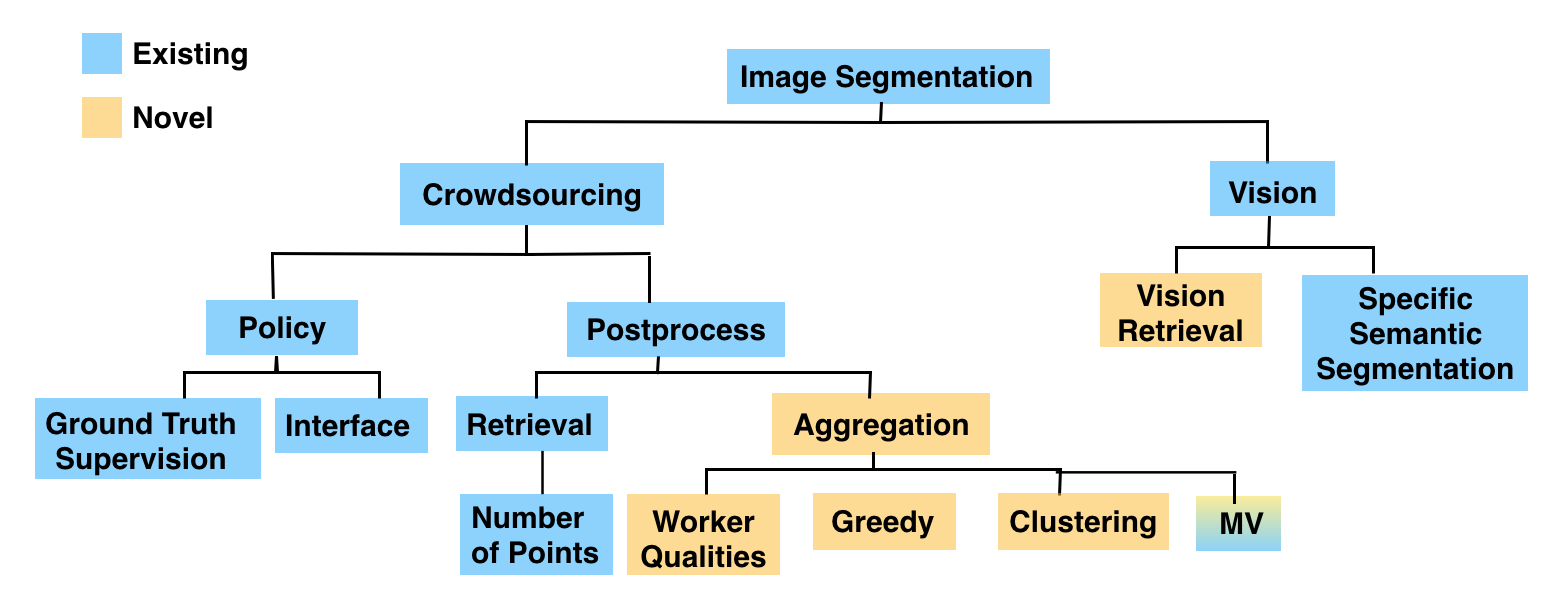
\includegraphics[width=\linewidth]{plots/flowchart.png}
\caption{Flowchart summarizing the classes of existing algorithms for image segmentation (blue) and a novel class of algorithms proposed in this paper (yellow). Majority-vote (MV) is colored both blue and yellow, since a common algorithm in crowdsourcing literature, but have not been extensively applied to crowdsourced image segmentation.}
\vspace{-10pt}
%The crowdsourced approach can be largely classified as retrieval or aggregation-based methods. We further explore hybrid algorithms that makes use of signals that span over multiple categories, described in our technical report.
\label{flowchart}
\end{figure}
%Many large-scale efforts in crowdsourced image segmentation contain little to no information on the quality characterization and evaluation of the collected dataset~\cite{Torralba2010,MartinFTM01,Li2009,Gurari2015}, which indicate the lack of standardized approaches for quality evaluation. 
As shown in Figure \ref{flowchart}, quality evaluation methods for crowdsourced segmentation can be largely classified into two categories:

\stitle{Retrieval-based methods} seek to pick the ``best'' worker segmentation based on some scoring criteria that evaluates the quality of each segmentation, including the use of vision information~\cite{Vittayakorn2011,Russakovsky2015}, expectation-maximization (EM) approaches for bounding box quality estimation~\cite{MDWWelinder2010}, and click-stream behavior \cite{Cabezas2015,Sameki2015,Sorokin2008}.

\stitle{Aggregation-based methods} use multiple worker segmentations to produce a single combined segmentation. %Our paper formulate a novel ``tiles'' approach for aggregation methods that operates on discrete non-overlapping units composed of all worker segmentations overlaid on top of each other. 
\ads{reword a bit to emphasize difference from retrieval; Aggregation-based methods combine multiple worker segmentations to produce a final segmentation, and are not restricted by any single worker segmentation.}
Aggregation-based majority vote have been introduced in Sameki et al. (\citeyear{Sameki2015}) as a way for aggregating expert segmentations to obtain a ground truth segmentation for evaluation purposes. \ads{Not clear how what they did is different from us---important to reword so that novelty of our aggregation methodology (and MV algo in particular) is not questioned.}

%specialized segmentation interfaces or workflows that ensures that the annotations collected are of high quality, including 
Orthogonal methods to improve segmentation quality include periodic verification workflows~\cite{Lin2014,Everingham15}, specialized segmentation interfaces~\cite{Song2018}, and vision-based supervision of crowdsourced segmentation\cite{Russakovsky2015,Gurari2016}. Our paper do not compare against these methods since they are not easily reproducible and could be used for quality improvement on top of any of the algorithms described in this paper.  %Since these policy-based methods are interface-dependent, require expensive expert-drawn ground-truth annotations or vision information, the results are not easily reproducible. In addition, the segmentations collected by the simple click-and-draw interface in many of the large scale segmentation efforts can not be improved with this technique as a post-processing method. Due to the lack of reproducibility, our paper do not compare against these policy-based methods in extensive details.


          \section{Preliminaries}
\subsection{Data \& Goals}
We collected crowdsourced segmentation data from Amazon Mechanical Turk where each HIT consisted of one segmentation task for a specific pre-labeled object in the image. There were a total of 46 objects in 9 images from the MSCOCO dataset~\cite{Lin2014}. For each object, we collected segmentation masks from a total of 40 workers. As shown in Figure \ref{interface}, each task contains a semantic keyword and a pointer indicating the object to be segmented. These tasks represent a diverse set of task difficulty (different levels of clutteredness, occlusion, lighting) and levels of task ambiguity. %Given a raw 
\subsection{Evaluation Metrics}
\par Evaluation metrics used in our experiment measures how well the final segmentation (S) produced by these algorithms compare against ground truth (GT). The most common evaluation metric used in literature are area-based methods which take into account the intersection, $IA=area(S\cup GT)$, or union, $UA=area(S\cap GT)$, between the user and the ground truth segmentations. Specifically, we use
    $\text{Precision (P)} = \frac{IA(S)}{area(S)}$, 
    $\text{Recall (R)} = \frac{IA(S)}{area(GT)}$, and 
    $\text{Jaccard (J)} = \frac{UA(S)}{IA(S)}$
    metrics to evaluate our algorithms.
 \techreport{\par A sub-sampled dataset was created from the full dataset to determine the efficacy of these algorithms on varying number of worker responses. Every object was randomly sampled worker with replacement. For small worker samples, we average our results over larger number of batches than for large worker samples (which have lower variance, since the sample size is close to the original data size).}
          %!TEX root = main.tex
% \section{Data}
\subsection{Data Collection\label{sec:data}}
We collected crowdsourced segmentation data 
from Amazon Mechanical Turk where each 
HIT consisted of one segmentation task 
for a specific pre-labeled object in the image. 
There were a total of 46 objects in 9 images from the MSCOCO dataset~\cite{Lin2014}. For each object, we collected segmentation masks from a total of 40 workers.  Each worker was paid 5 cents per annotation. After eliminating segmentation masks that contains self-intersecting polygon contours, our final dataset contains 1784 bounding boxes made by 198 unique workers. As shown in Fig.\ref{interface}, each task contains a semantic keyword and a pointer indicating the object to be segmented. These tasks represent a diverse set of task difficulty (different levels of clutteredness, occlusion, lighting) and levels of task ambiguity. 
\begin{figure}[ht!]
\centering
\fbox{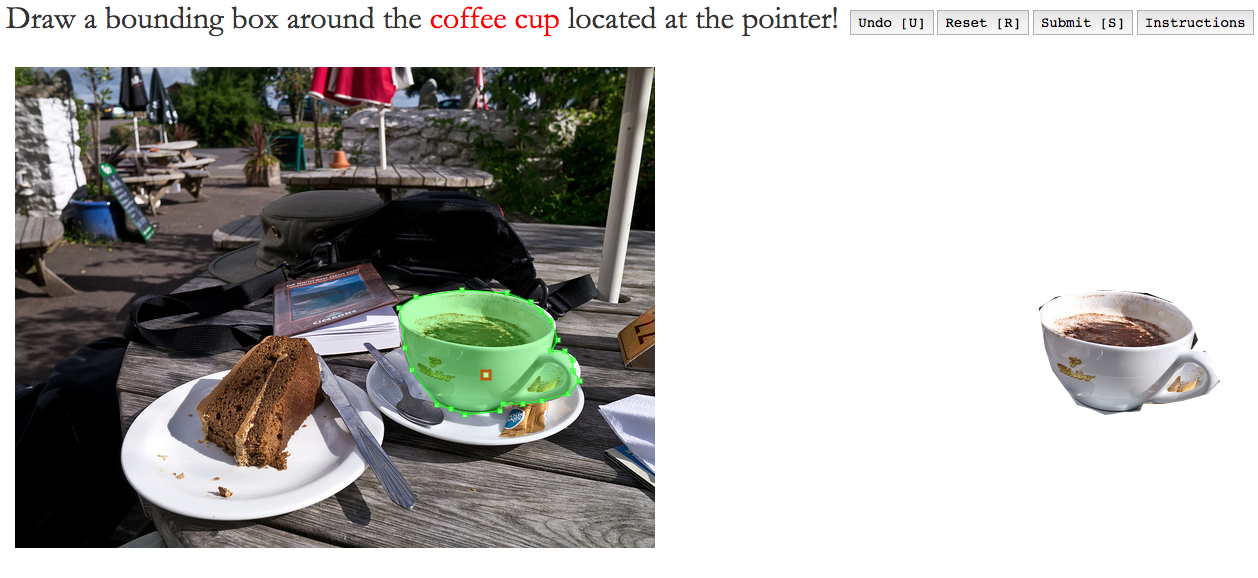
\includegraphics[width=0.9\linewidth]{plots/interface.png}}
\caption{An example interface for the segmentation webapp can be seen  \href{http://crowd-segment.herokuapp.com/segment/COCO_train2014_000000000127/10/}{here}.}
\label{interface}
\end{figure}
% We eliminated all bounding boxes \agp{likewise} from workers that were self-intersecting\agp{not clear}. 

\subsection{Worker Error patterns\label{sec:errors}}
\par Raw data collected from crowdsourced image processing tasks are known to be noisy due to varying degrees of worker skills, attention, and motivation~\cite{bell14intrinsic,MDWWelinder2010}. The average precision, recall and Jaccard similarity of the worker segmentation against the ground truth across all of the objects was 92\%, 94\%, 86\% respectively. While workers have equal rates of overbounding or underbounding behavior, workers tend to overbound by a larger amount (7212 pixels on average) than underbound (1306 pixels on average). %The distributions of worker's bounding box qualities approximately follows a transformed Gaussian (Johnson SU) distribution that accounts for the right-skewed, long-tail characteristics of the distribution\agp{this comes out of nowhere; also simplify}.
\par Visual examination of worker bounding boxes reveals several common error patterns evident across different objects. As shown in the example in Figure \ref{error_examples}, common worker errors can be classified into three types:
\begin{enumerate}
	\item \textbf{Semantic error:} Workers annotate the wrong semantic object.
	\item \textbf{Regional semantic ambiguity:}Workers annotate the correct semantic object, but included a portion connected to that object that should not have been included as part of the annotation.
	\item \textbf{Boundary imprecision:} Workers annotate the correct semantic object, but segmentation boundaries are imprecise. %(obj 17) \agp{where did obj 7 come from? point to image}
\end{enumerate}
Type 1 and 2 errors have also been observed in prior work~\cite{Sorokin2008,Lin2014,Gurari2018}, which noted that disagreement in worker responses can come from questions that are ambiguous or difficult to answer, such as segmenting a individual person from a crowd. Since there are multiple workers annotating each object, each object can suffer from multiple types of error: we found that out of the 46 objects in our dataset, 9 objects suffer from type one error and 18 objects from type two error. Almost all objects suffer from some form of type three error of varying degree of imprecision around the object boundary. The main evaluation methods highlighted in this paper focuses on resolving the type three imprecise, ``sloppy'' bounding box errors. However, since type one and two errors are also fairly severe in contributing to the recall lost, we did not want to simply eliminate objects that suffer from these issues. We will discuss a preprocessing procedure used to address these errors in Section~\ref{sec:methods}.

\agp{after having read all this, i wonder if we want to simply move the dataset description to when the evaluation happens; here just say that we look at some example worker segmentations for some tasks that we issued and try to identify general principles that can motivate the design of the algorithms, described next.}\dor{No, I agree that this would help highlight these observation as one of our contribution, this section needs to appear early on, to motivate why we have developed certain algos for resolving perspectives (e.g. clustering)}
          %!TEX root = main.tex
\section{Perspective Resolution in Crowdsourced Image Segmentation}
\subsection{Worker Clustering}
Our clustering-based approach is based on the intuition that workers with similar perspectives  will have segmentations that are closer to each other, while workers with different perspectives from each other will have segmentations that differ from each other. We capture the similarity between a pair of workers by computing the Jaccard score between their segmentations and perform {\em spectral clustering} to separate workers into clusters. Figure \ref{cluster_example} illustrates how spectral clustering is capable of dividing the worker responses into clusters with meaningful semantic associations, reflecting the crowd's diversity of perspectives in completing same task.
    \begin{figure}[ht!]
      \centering
      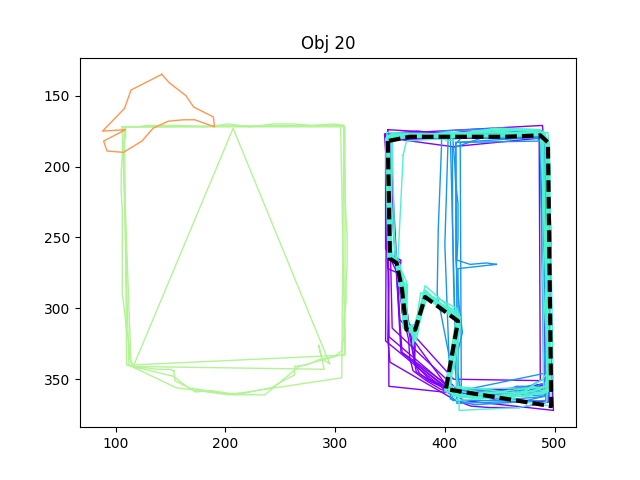
\includegraphics[width=\textwidth]{plots/20.png}
      \caption{Example image showing clustering performed on the same object from Figure \ref{error_examples}.}
      \label{cluster_example}
    \end{figure}
\par Clustering results can also be used as a preprocessing step to any of the quality evaluation algorithms by keeping only the segmentations that belong to the largest cluster, which is typically free of any semantic errors. As shown in Table~\ref{statsTable}, on average, clustering generally results in an increase the resulting algorithmic performance. Since the ground-truth supervised variants are already free of semantic ambiguity and errors, there is minimal improvement resulting from clustering. %In particular, we see a greater improvement with clustering preprocessing for algorithms that are not very robust in resolving semantic errors or ambiguity, such as for the \texttt{num pts} retrieval algorithm, than compared to the aggregation-based methods. 
\par Clustering offers an additional benefit of preserving worker's semantic intentions in the case where there are multiple instances of different errors. For example, in Figure \ref{cluster_example}, the mistakened clusters included semantic concepts ``monitor'' and ``turtle''. While these are considered \textit{bad} annotations for this particular task, this cluster of annotation can provide more data for another semantic segmentation task ``monitor''. A potential direction of future work includes adding an additional crowdsourcing task for semantic labelling of clusters (which is cheaper and more accurate than segmentation) to enable reuse of annotations across objects and lower the cost of data collection. 
          \section{Aggregation Methods: A Closer Look~\label{sec:agg-detailed}}
%Describe Tile based models. Briefly describe construction of tiles from BBs.
% In this section we formalize the problem of picking an optimal set of tiles, and describe our solution to this problem.
% \subsection{Definitions}
The key insight of aggregation-based methods is that they perform inference at a more fine-grained ``tile'' level, rather than at the bounding box level as is in the case of retrieval-based methods. In this section, we discuss three different algorithms for choosing a ``good'' set of worker tiles in aggregation-based methods.
%In this section, we discuss aggregation based methods which use combine the segmentations from multiple workers and output a single merged segmentation. As described earlier in Section~\ref{sec:crowd}, our aggregation algorithms first transform the set of worker segmentations into tiles, as shown in Fig.~\ref{tile_demo}, and then choose a set of tiles to include in the final segmentation. \todo[inline]{modify figure, or use from prev section if added.} Since aggregation based approaches work at the level of tiles, they are more fine-grained than retrieval-based methods, which work at the granularity of complete worker segmentations.
\begin{figure}
\centering
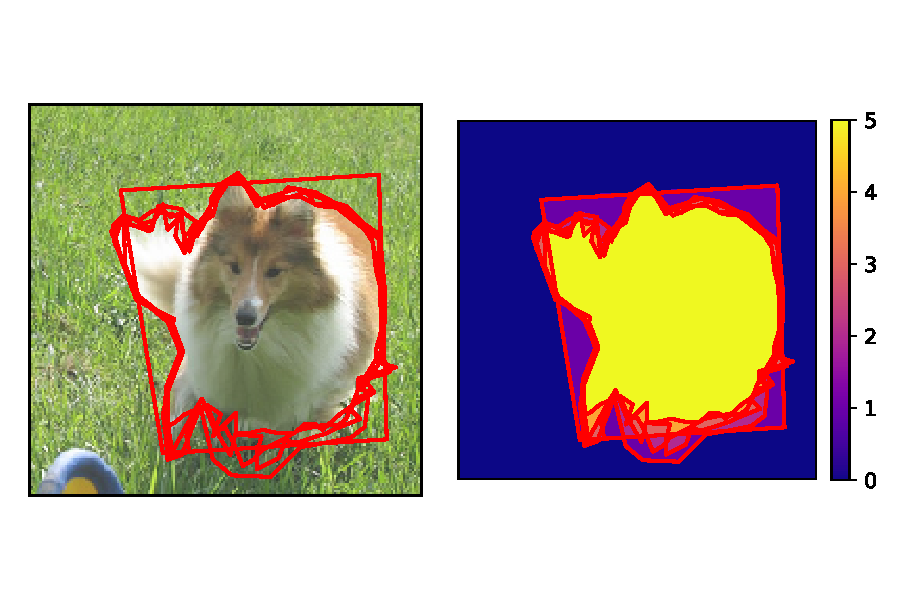
\includegraphics[width=\textwidth]{plots/tile_demo.pdf}
\caption{Left: Red boundaries shows the segmentation boundaries drawn by five workers overlaid on the image. Right: Segmentation boundaries still shown in red. The overlaid segmentation creates a masks where the color indicates the number of workers who voted for the tile region.}
\label{tile_demo}
\end{figure}
% \begin{figure}
% \centering
% 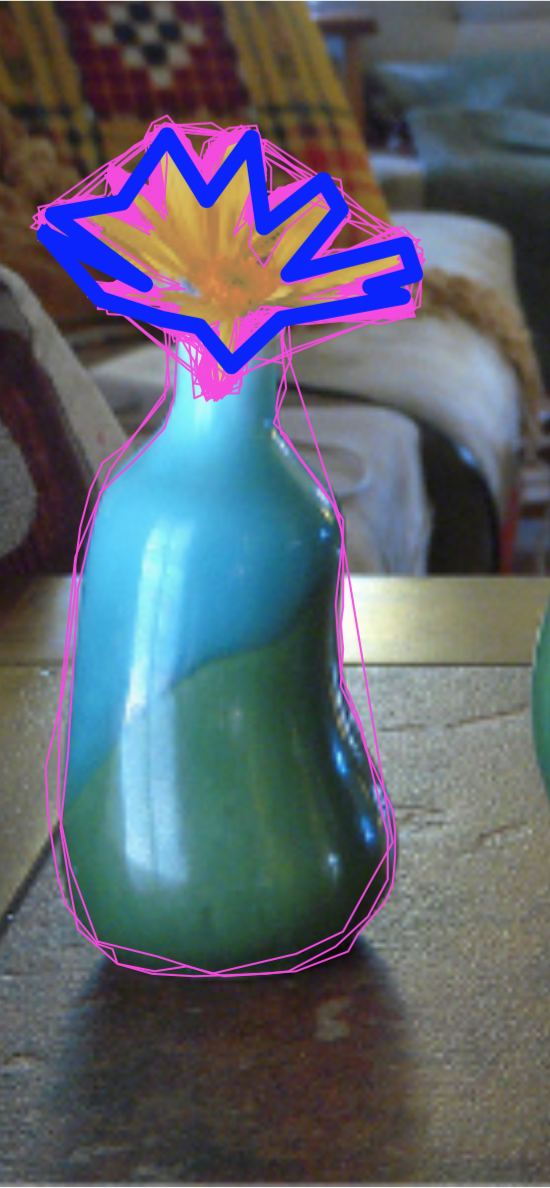
\includegraphics[width=.25\textwidth]{plots/worker_cropped.png}
% 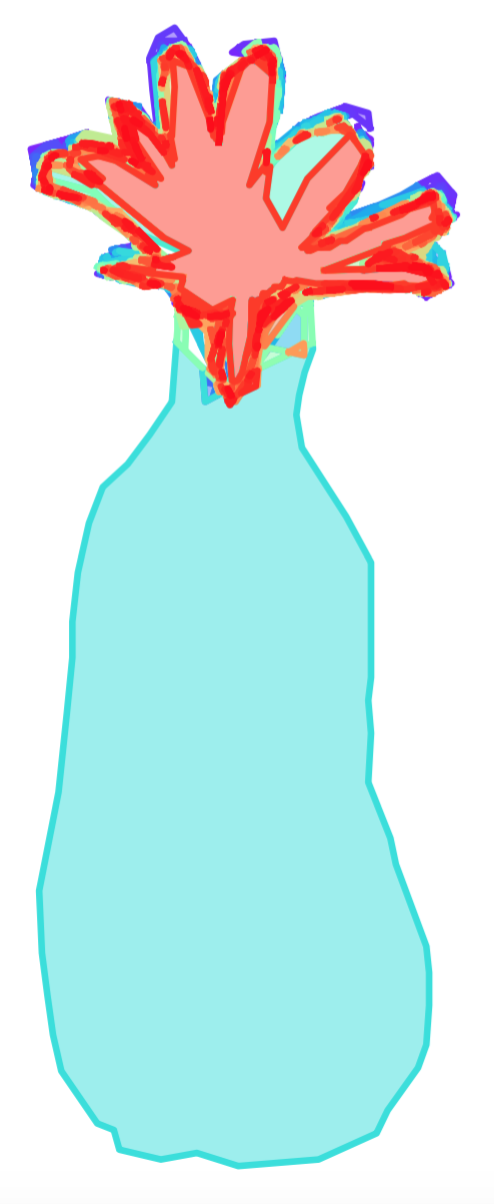
\includegraphics[width=.2\textwidth]{plots/tile_cropped.png}
% 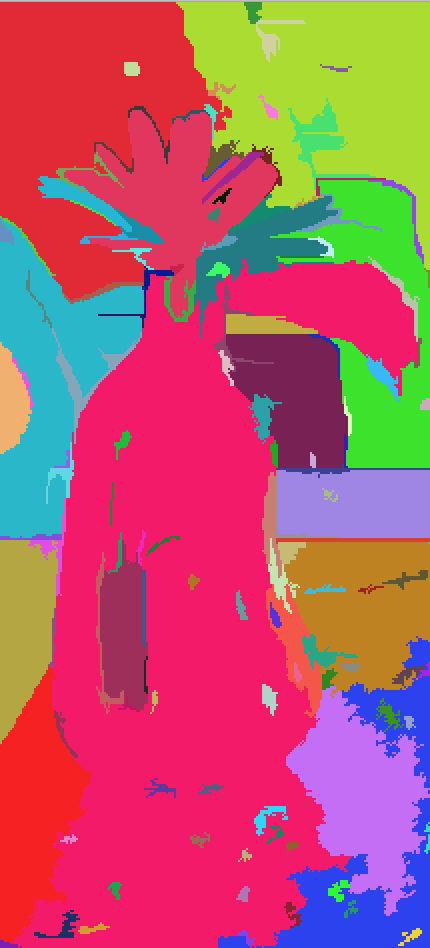
\includegraphics[width=.25\textwidth]{plots/vision_cropped.png}
% \caption{Left: Pink shows 40 worker bounding boxes for the object ``flower'' and blue ground truth segmentation, superimposed on the original COCO image. Center: Non-overlapping tiles constructed from worker bounding box. Right: Output from the color-segmentation vision algorithm.}
% \label{flower_example}
% \todo[inline]{Add black and white, vision segmented region image}
% \end{figure}
%Clarify that our search space is tile combination formed by all the worker's tiles not the space of all possible coordinates. (i.e. we assume that a region can not be inside the BB if no workers bounded that region)

\subsection{Majority Vote Aggregation (MV)}
A common strategy for aggregating multiple worker responses in crowdsourced algorithms is {\em Majority Vote}(MV)\dor{Akash: add citation for MV from general crowdsourcing domain}. In the context of choosing worker tiles to produce a segmentation, the natural Majority Vote algorithm looks at each tile, and includes the tile in the output segmentation if and only if the tile is covered by at least 50\% of all worker segmentations.
% We investigated three types of variants for majority vote strategies: picking the top-k, top-percentile tiles of vote counts and picking the tiles that were voted by at least 50\% of the workers. We found that among these majority vote variants, the latter strategy gave the highest accuracy.

\subsection{Expectation-Maximization}
While Majority Vote is a very useful algorithm in practice, it does not distinguish between workers in any way. In reality, however, not all workers are equal. Now, we try to model worker quality, and use worker quality information to infer the likelihood that a tile is part of the ground truth segmentation. 
Since both, the worker qualities, as well as the likelihoods of tiles being part of the ground truth are hidden quantities, we employ an Expectation-Maximization based approach to simultaneously esimtate both of these sets of quantities. 
\todo[inline]{techreport}
\papertext{We intuitively describe three worker models that we experiment with below. In our technical report, we formalize the notion of the probability that a set of tiles forms the ground truth, and solve the corresponding maximum likelihood problem, for each of these worker models. }

\subheading{Worker quality models.}
We can think of workers as agents that look at each pixel in an image and label it as part of the segmentation, or not. Their actual segmentation is the union of all the pixels that they labeled as being part of their segmentations. Each pixel in the image is also either included in the ground truth segmentation or not included in the ground truth segmentation. We can now model worker segmentation as a set of boolean pixel-level (include or don't include) tasks, each having a ground truth boolean value. Based on this idea, we explore three worker quality models:
\begin{itemize}
\item {\em Basic model:} Each worker is captured by a single parameter Bernoulli model, $<q>$, which represents the probability that a worker will label an arbitrary pixel correctly.
\item {\em Ground truth inclusion model (GT):} Two parameter Bernoulli model $<qp, qn>$, capturing false positive and false negative rates of a worker. This helps to separate between workers that tend to overbound and workers that tend to underbound segmentations.
\item {\em Ground truth inclusion, large small area model (GTLSA):} Four parameter model $<qp_l, qn_l, qp_s, qn_s>$, that distinguishes between false positive and false negative rates for large and small tiles. In addition to capturing overbounding and underbounding tendencies, this model captures the fact that workers tend to make more mistakes on small tiles, and penalizes mistakes on large tiles more heavily.
\end{itemize}


\subsection{Greedy Tile Picking}\dor{the terminology ``overlap'' can be a bit confusing with the abbrev that we chose, since overlap area would be OA (rather than outside area). Maybe introduce it as intersection area or introduce terms ``inside'' and ``outside'' to correspond with the abbrev OA,IA.}
Next, we present a greedy tile picking algorithm that grows the output set of tiles by adding in one tile at a time. Suppose tile $t$, overlaps with the ground truth segmentation with intersection area of $IA(t)$, and has area $OA(t)$ not overlapping with the ground truth. The greedy algorithm sorts tiles in decreasing order of their $\frac{IA(t)}{OA(t)}$ ratio and iteratively adds the next tile to the growing set of output tiles, until the Jaccard value of the current set of tiles will decrease with the next added tile. \dor{explain intuition of why I/O is used.} The key idea behind this algorithm is the following statement\papertext{\todo[inline]{techreport}(proof available in our technical report)}: It can be shown that given a set of tiles, $T$, the tile $t$ that maximizes Jaccard($T\cup t$) score of the union of the set of tiles against the ground truth, is the tile with maximum value of $\frac{IA(t)}{OA(t)}$. The primary challenge with this approach is that we do not know the actual $IA(t)$, $OA(t)$ values for any tile. We implement a heuristic version of this algorithm, where we estimate the intersection area of any tile, $IA(t)$, by using the fraction of workers that have voted for a tile, and greedily maximize for estimated Jaccard value at every step. \papertext{\todo[inline]{techreport}In our technical report, we also discuss variants of this algorithm where we use different techniques to estimate the intersection areas of tiles, resulting in corresponding variants of the greedy algorithm.}


\techreport{
% begin techreport
Tiles are finer grained than bounding boxes. Our tile-based approach is inspired by the S-T graph in the classical graph cut problem, where the goal of image segmentation is to find a vertex partition between the object and background regions.\todo[inline]{we don't actually use tile graph here, move to vision section? }

\par $\mathcal{T}=\{t_k\}$ is the set of all non-overlapping tiles for an object i. T is the ground truth tile set. $T^\prime$ is some combination of tiles chosen from $\mathcal{T}$.
 The indicator label $l_{kj}$ is one when worker j votes on the tile $t_{k}$ (i.e. the bounding box that he draws contains $t_{k}$), and zero otherwise. The indicator matrix consisting of tile indicator for all workers is denoted as $\mathbf{l_{kj}}$.

\subsection{Worker Error Model}
We propose three different worker error models describing the probability of a worker j's vote on a specific tile $t_k$, given the tile's inclusion in ground truth and a set of worker qualities $Q_j$. 
\begin{enumerate}
\item Basic: single-parameter Bernoulli model, where $q_j$ is the probability of the worker getting a tile correct. A worker is correct when his vote ($l_{jk}$) matches with the ground truth inclusion of the tile ($t_k\in T$). A worker makes an incorrect response when their vote contradicts with the inclusion of the tile in T ($\{t_k\in$ T$\quad\&\quad l_{kj}=0\}, \{t_k\notin $T$\quad\&\quad l_{kj}=1\}$)
\begin{equation}
p(l_{jk}|t_k\in T, Qj) = \begin{cases}
               q_j, \quad l_{jk}=1\\
               1-q_j, \quad l_{jk}=0\\
            \end{cases}
\end{equation}
\item Large Small Area (LSA): The basic model equally weighs all tiles, but intuitively a worker should be rewarded more if they get a large-area tile correct. We use a two-parameter Bernoulli to model two different tile sizes determined by a threshold $A^*$.
\begin{equation}
p(l_{jk}|t_k\in T,Q_j) = \begin{cases}
               q_{j1}, \quad l_{jk}=1 \& A(t_k)\geq A^*\\
               1-q_{j1}, \quad l_{jk}=0 \& A(t_k)\geq A^*\\
                q_{j2}, \quad l_{jk}=1 \& A(t_k)< A^*\\
               1-q_{j2}, \quad l_{jk}=0 \& A(t_k)< A^*\\
            \end{cases}
\end{equation}
\item Ground truth inclusion, large small area (GTLSA): We observe in our experiment that there can be many large area tiles that lies outside of the ground truth drawn by workers who tend to draw loose, overbounding boxes. Our 4 parameter Bernoulli model distinguishes between false and true positive rates, by taking into account the positive and negative regions (i.e. regions that lies inside or outside of T). 
In the case where $A(t_k)\geq A^*$: 
\begin{equation}
p(l_{jk}|t_k\in T,Q_j) = \begin{cases}
               q_{p1}, \quad l_{jk}=1  \\
               1-q_{p1}, \quad l_{jk}=0  \\
            \end{cases}
\end{equation}
\begin{equation}
p(l_{jk}|t_k\notin T,Q_j) = \begin{cases}
               q_{n1}, \quad l_{jk}=0  \\
               1-q_{n1}, \quad l_{jk}=1  \\
            \end{cases}
\end{equation}
%\item Area-weighted scoring: 
From the worker error model, we can also derive the probability that a tile is in ground truth $p(t_k\in T|Q_j, l_{jk})$ using Bayes rule, assuming the prior probabilities as constant.
\end{enumerate}

\subsection{Problem Statement}
%Describe assumptions on pdfs and inference process. (E and M steps). How are parameters in the models determined empirically.
\par For our problem, we consider only finding tile regions that could be constructed from worker bounding boxes. In other words, our objective is to find the tile combination $T^\prime$ that maximizes the probability that it is the ground truth p($T^\prime$=T), given a set of worker qualities $Q_j$ and tile indicator labels $l_{jk}$: 

\begin{equation}
T = \argmax_{T^\prime \subseteq \mathcal{T}}p(T=T^\prime |  \mathbf{l_{kj}},Q_j)
\label{objective}
\end{equation}
Using Bayes rule we can rewrite this in terms of the posterior probability of the tile-based values($\mathbf{l_{kj}}$) or worker-based values($Q_{j}$), which we can use for the E and M step equations respectively. 
\subsection{Inference}
\par For the E step, we assume T' is ground truth and estimate the $Q_j$ parameters. We can rewrite Eq.\ref{objective} as: 
\begin{equation}
p(T^\prime| Q_j,\mathbf{l_{kj}})
\approx p(l_{kj}| Q,T^\prime)
\end{equation}
where we treat the priors $p(T^\prime),p(Q_j)$ as constants.
Our goal is to find the maximum likelihood parameters of $Q_j$: 
\begin{equation}
\hat{Qj} = \argmax_{Q_j} p(Q_j| \mathbf{l_{kj}},T^\prime)
\end{equation}
% assume p(T') uniform or constant p(Qj), no prior information 
We use the binary random variable w to indicate whether the worker makes a correct vote (w=1) or an incorrect vote(w=0) for a tile. We can write the worker quality probability as the product of the probabilities that they would assume these two independent states (correct/incorrect). 
\begin{align}
p(Q_j) = \prod_j q_j^{p_j(w=1)}\cdot [1-q_j]^{p(w=0)}
\end{align}
The closed form of the maximum likelihood solution for the Bernoulli distribution reduces down to: 
\begin{equation}
\hat{q_j}=\frac{n_{correct}}{n_{total}}
\end{equation}
\par For the M step, we maximize the likelihood of the tile combination $T^\prime$ for a fixed set of worker qualities, $\{Q_j\}$. Following Eq.\ref{objective} from Bayes rule, 
\begin{equation}
p(T^\prime| Q_j,\mathbf{l_{kj}})
\approx p(\mathbf{l_{kj}}|Q_j,l_k)
\end{equation}
% rephrase what your optimization function is, i.e. argmax RHS of equation p(lkj)
Our optimization function is written as:
\begin{equation}
\hat{T^\prime}=\argmax_{T^\prime\supseteq \{T^\prime\} } \prod_j p(\mathbf{l_{kj}}|Q_j,l_k)
\end{equation}
 The product over $T^\prime$ can be further decomposed into its tile components. The likelihoods of these tiles can be computed via the worker error model: 
\begin{equation}
=\argmax_{T^\prime\supseteq \{T^\prime\}} \prod_j\Bigg[\prod_{t_k\in T^\prime} p(t_k\in \mathrm{T}|Q_j,l_k)\prod_{t_k\notin T^\prime} p(t_k\notin \mathrm{T}|Q_j,l_k)\Bigg]
\end{equation}
% * <akashds.iitk@gmail.com> 2017-04-25T02:53:10.683Z:
% 
% The term summing over, $T' \subsetof \mathbf{T} $ can have slightly better notation. Introduce some bold T as space of all possible tile combinations, and use T' subsetof T.
% 
% ^.
\subsubsection{NP-hardness proof}
\subsection{Optimization}
%Explain heuristics used for avoiding to search through all T'. 
Since the space of possible $\{T^{\prime}\}$ to search through is $2^{N}$ where number of tiles (N) for an average object with 30$\sim$40 worker is on the order of thousands, we develop several strategies to narrow the search space for making the problem computationally feasible. 
\subsubsection{High-confidence snowball}
The goal of the snowball method is to come up with smaller subsample of tile combinations $T^\prime$ that are good candidates of ground truth. First, we use tile properties such as area or votes as a heuristic to derive a fixed set of high-confidence tiles as the core. Then, using the same heuristic, we randomly generate subsets from other medium confidence tiles and combined with these core tiles. Tiles picked with such heuristics often have high recall, which means that our TileEM algorithm essentially helps us find a more precise $T^{\prime}$ from $\{T^{\prime}\}$. In our experiment, we define our confidence score as 2$\cdot$votes+area, with 3 high-confidence, fixed core tiles and 40 flexible medium confidence tiles. 
\todo[inline]{NOTE: Might want to consider adjacency-based snowball approach too}
\subsubsection{Maximum likelihood Construction}
Apart from constructing a set of  $\{T^{\prime}\}$ for picking the best  $T^{\prime}$, we can instead directly construct the maximum likelihood tile $T^*$ by choosing tiles that satisfy the criterion: 
\begin{equation}
T^* = \{t_k|p(t_k\in T|l_k,Q_j)\geq p(t_k\notin T|l_k,Q_j)\}
\end{equation}
\subsubsection{Proof:}
We show that this tile-picking heuristic is at least as likely as any tile combination that we would pick with the $\{T^{\prime}\}$ selection method. Suppose there is a $T^\prime$ such that it consists of the same tiles as $T^*$, but we randomly drop a tile $t_{k^\prime}$
\begin{equation}
p(T^*=T^\prime|l_k,Q_j)=\prod_{t_k} p(t_k\in T^*)\cdot p(t_{k^\prime}\notin T^*)
\end{equation}
By definition all tiles in $T^*$ must satisfy $p(t_k\in T|l_k,Q_j)\geq p(t_k\notin T|l_k,Q_j)$, so the dropped tile must have lower probability than $T^\prime$.
\begin{align}
p(T=T^\prime)=p(T^*\setminus t_k^\prime) p(t_k^\prime \notin T^*) \\
% * <akashds.iitk@gmail.com> 2017-04-25T03:02:53.207Z:
% 
% > T^*
% T'
% 
% ^.
p(T=T^*)=p(T^*\setminus t_k^\prime) p(t_k^\prime \in T^*) 
\end{align}
By dropping multiple $t_{k^\prime}$ from $T^*$ or adding $t_{k^\prime}$ not previously in $T^*$, the above result can be generalized to arbitrary $T^\prime$.
\begin{algorithm}[ht!]
 \KwData{fixed $Q_j$}
 %\KwResult{}
 Initialize $T^*$\;
 \For{$t_k \in \mathcal{T}$ }{
  \If{$p(t_k\in T)\geq p(t_k\notin T)$ }{
   $T^*\leftarrow T^* \cup t_k$;
   }
 }
 \caption{M step algorithm. For the initialization of $T^*$, we could start from either an empty set or a high-confidence tileset. The set of $\mathcal{T}$ to chose from can either be the set of all tiles or all tiles adjacent to $T^*$. }\label{Mstep}
\end{algorithm}

\subsection{Our Algorithm}
\todo[inline]{name / abbreviation for algo}
In practice, we desire contiguous bounding boxes. Therefore, we impose an adjacency constraint while choosing our set of optimal tiles. Furthermore, we find that we can trade-off precision for recall by relaxing our condition for choice of tile \todo[inline]{p(tk) $>=$ thresh}.
\begin{algorithm}[ht!]
 \KwData{fixed $Q_j$}
 %\KwResult{}
 $T^*$ = high confidence tiles\;
 $d^\prime$=0\;
 good tile count at $d^\prime$=1\;
 \While{good tile count at $d^\prime \neq 0$}{
    $\{t_{k,d=d^\prime}\}\leftarrow$ find all tiles at d=$d^\prime$ shell\;
    \For{$t_k \in \{t_{k,d=d^\prime}\}$}{
        \If{$p(t_k\in T)\geq p(t_k\notin T)$ }{
            $T^*\leftarrow T^* \cup t_k$\;
            good tile count at $d^\prime$ ++\;
        }    
    }
    $d^\prime$++\;
 }
 \caption{Shell-based M step algorithm enforces tiles that are added into $T^*$ must be adjacent to one another.}\label{Mstep}
\end{algorithm}

% end techreport
}
          \section{Experimental Results\label{sec:experiment}}
\subsection{Aggregation-based methods perform significantly better than retrieval-based methods (no clustering)}
\begin{figure}[h!]
   \centering
   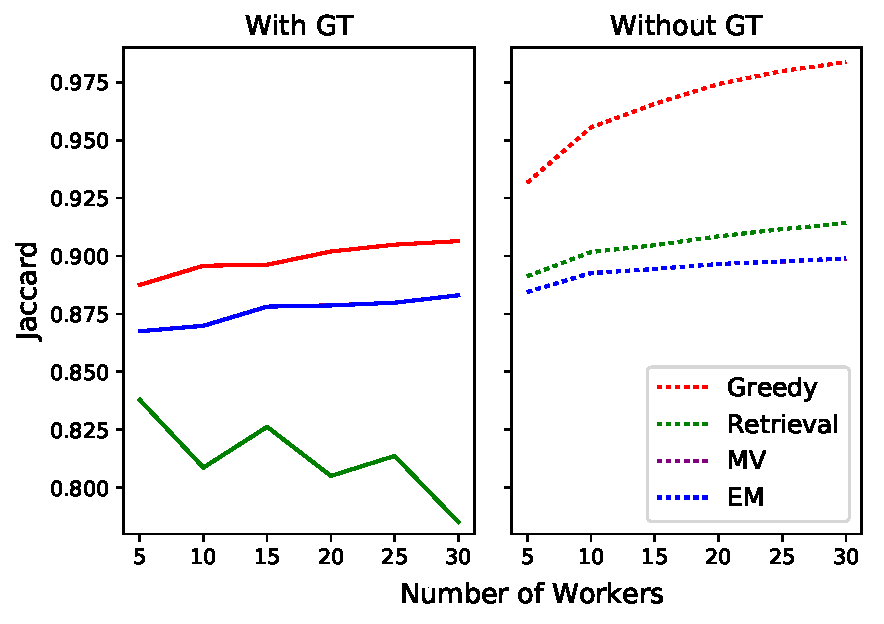
\includegraphics[trim={0 1pt 4pt 0},clip,width=0.8\linewidth]{plots/Retrieval_vs_Aggregation.pdf}
   \caption{Performance of the original algorithms that do not make use of ground truth information (Left) and ones that do (Right). MV and EM results are so close that they overlay on each other.} 
   \label{retrieval_vs_aggregation}   
\end{figure} 
\npar In Figure~\ref{retrieval_vs_aggregation}, we vary the number of worker segmentations along the x-axis and plot the average Jaccard score on the y-axis across different worker samples of a given size across different algorithms. Figure~\ref{retrieval_vs_aggregation} (left) shows that the performance of aggregation-based algorithms (greedy, EM) exceeds the best-achievable through existing retrieval-based method (Retrieval). Then, in Figure \ref{retrieval_vs_aggregation} (right), we estimate the upper-bound performance of each algorithm by assuming that the `full information' based on ground truth was given to the algorithm. For greedy, the algorithm is aware of all the actual tile overlap and non-overlap areas against ground truth, and does not need to approximate these values. For EM, we consider the performance of the algorithm if the true worker quality parameter values (under our worker quality model) are known. For retrieval, the full information version directly picks the worker with the highest Jaccard similarity with respect to the ground truth segmentation. By making use of ground truth information (Figure~\ref{retrieval_vs_aggregation} right), the best aggregation-based algorithm can achieve a close-to-perfect average Jaccard score of 0.98 as an upper bound, far exceeding the results achievable by any single `best' worker (J=0.91). This result demonstrates that aggregation-based methods are able to achieve better performance by performing inference at the tile granularity, which is guaranteed to be finer grained than any individual worker segmentation. 

\subsection{The performance of aggregation-based methods scale well as more worker segmentations are added.}
\par \noindent Intuitively, larger numbers of worker segmentations result in finer granularity tiles for the aggregation-based methods. The first row in Table~\ref{statsTable} lists the average percentage change in Jaccard between 5-workers and 30-workers samples, demonstrating a monotonically increasing relationship between number of worker segmentations used and the performance. However, retrieval-based methods do not benefit from more segmentations.

\subsection{Clustering as preprocessing improves algorithmic performance.}
\par \noindent The average percentage change between the no clustering and clustering results is shown in Table~\ref{statsTable}. Clustering generally results in an accuracy increase. Since the `full information' variants are already free of semantic ambiguity and errors, clustering does not assist with further improvement. %In particular, we see a greater improvement with clustering preprocessing for algorithms that are not very robust in resolving semantic errors or ambiguity, such as for the \texttt{num pts} retrieval algorithm, than compared to the aggregation-based methods. 
\begin{table}[h!]
     \small
     % \setlength\tabcolsep{1.5pt}
     \scalebox{0.85}{
      \begin{tabular}{l|l|l|l|l|l|l|l}
      & \multicolumn{3}{c|}{Retrieval-based} & \multicolumn{4}{l}{Aggregation-based} \\ \hline
      Algorithm       & num pts     & worker    & worker*    & MV     & EM     & greedy   & greedy*   \\ \hline
      Worker Scaling    & -6.30       & -0.25     & 2.58       & 1.63   & 1.64   & 2.16     & 5.59      \\ \hline
      Clustering Effect & 5.92        & 4.00      & -0.02      & 2.05   & 1.38   & 5.55     & -0.06    
      \end{tabular}
      }
      \caption{Jaccard percentage change due to worker scaling and clustering. Algorithms with * makes use of ground truth information.}
      \label{statsTable} 
\end{table}
\par The clustering preprocessing step can significantly improve performance of algorithms that are not very robust to segmentations with semantic errors or ambiguities, such as the heuristic-based number of points approach. When examining the gap of increase with and without clustering in Figure \ref{cluster_effect}, we find that aggregation-based methods performs better than retrieval-methods exhibits a smaller gap between the performances. This effect is due to aggregation-based method's higher performance in the no cluster case, indicating that it is able to capture some of the semantic ambiguities and errors in the dataset.
\begin{figure}[ht!]
      \centering
      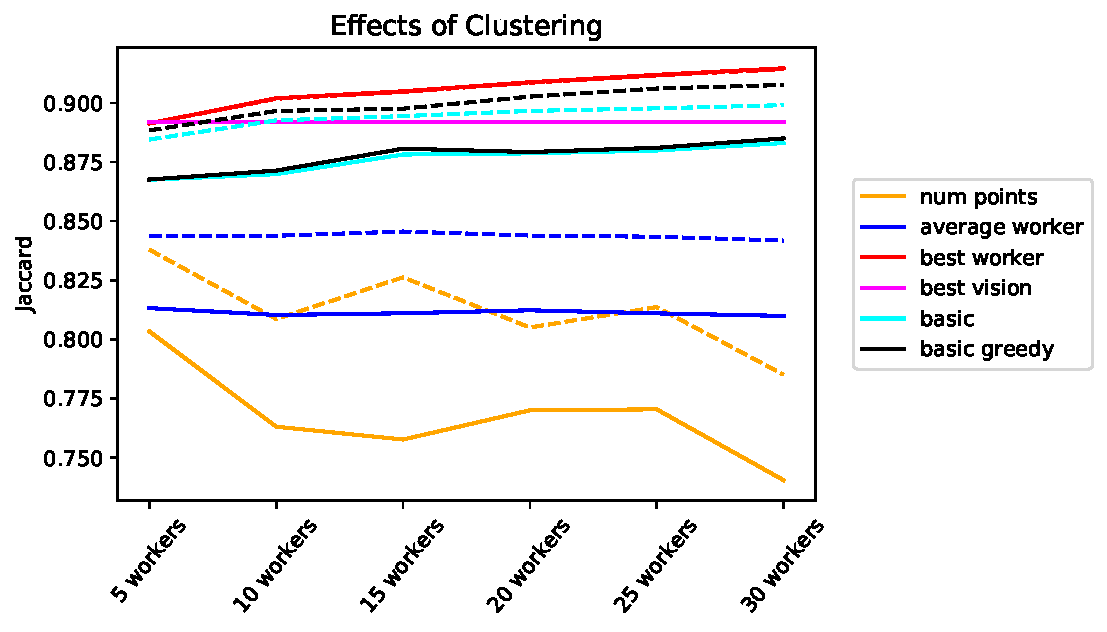
\includegraphics[width=\linewidth]{plots/Effects_of_clustering.pdf}
      \caption{Performance comparisons between averaging over experiments with clustering as a preprocessing step (dotted) and the unclustered results (solid) for different algorithms.}
      \label{cluster_effect}
\end{figure}
\subsection{How well does the inferred worker qualities predict individual worker performance?}
    \stitle{Correlation of worker qualities against performance}
     To further investigate how the EM models are performing, we looked at whether the model-inferred worker qualities is indicative of the actual quality of a segmentation. We performed linear fitting independently for each sample-objects and computed the $R^2$ statistics to determine whether worker qualities can accurately predict precision, recall, and Jaccard scores. Visual inspection of the basic worker quality model fitting showed that for objects that suffered from type two errors (semantic ambiguity), the single-parameter worker quality was unable to capture the overbounding behavior, which lead to a low precision and Jaccard. The results are listed in Table \ref{correlation} to highlight how our advanced worker qualities were able to better capture these scenarios. The clustering preprocessing was not performed for the values in Table \ref{correlation} to demonstrate the sole effect of the EM algorithm. Nevertheless, our clustered results also show a similar trend, with an average of $R^2$=0.88 and 0.89 for the GT and GTLSA models across all objects respectively. We also find that in general the linear fit improves as the number of data points increases, which indicates consistency in the fitted model.
    \begin{table}[ht!]
      \small
      \begin{tabular}{ccccccc}
        \hline
           N &   basic &   GT &   GTLSA &   isobasic &   isoGT &   isoGTLSA \\
        \hline
              5 &      0.601 &   0.907 &      0.901 &       0.576 &    0.907 &       0.904 \\
            10 &      0.632 &   0.895 &      0.899 &       0.633 &    0.895 &       0.898 \\
            15 &      0.622 &   0.897 &      0.898 &       0.622 &    0.897 &       0.897 \\
            20 &      0.636 &   0.894 &      0.899 &       0.637 &    0.894 &       0.898 \\
            25 &      0.66  &   0.901 &      0.905 &       0.661 &    0.901 &       0.904 \\
            30 &      0.673 &   0.907 &      \cellcolor{blue!25}0.914 &       0.676 &    0.907 &       \cellcolor{blue!25}0.913 \\
        \hline
      \end{tabular}
        \caption{Linear correlation of worker qualities against ground truth performance for different quality models across different number of workers (N). The lower worker samples exhibit lower $R^2$ due to the variance from smaller number of datapoints for each independent fit. }
        \label{correlation}
    \end{table}
    % \subsubsection{EM performance with different worker quality models}
    %   - why is iso cases not performing as well
    \stitle{Best worker quality retrieval}
    One application of worker qualities is that it could be used as an annotation scoring function for retrieving the best quality worker segmentation. We explore this approach by training a linear regression model for every sample-object and use the worker qualities to predict the precision, recall, and Jaccard of individual worker annotations against ground truth. Then, we query the model with the inferred worker quality and retrieve the worker with the best predicted Jaccard. 
    \par The reason why a linear regression model was chosen rather than simply sorting the worker qualities and picking the best is that sorting based on multiple worker qualities (precision, recall, Jaccard) effectively applies equal weighting to all quality attributes, whereas our advanced models are specifically designed to capture cases of false-positives and false-negatives that can yield drastically different recall and precision values. We have tested that the linear regression model performs better on this task that simple sorting is capable of learning the weights that helps it make better predictions. As shown in Table~\ref{bigtable}, the performance of worker-quality based retrieval is comparable the performance other aggregation-based methods. We find that amongst the different worker quality models, advanced worker quality models perform the best, agreeing with our intuition regarding correlation results observed in Table~\ref{correlation}.
    \begin{table}[ht!]
    \small
    \setlength\tabcolsep{3pt}
    \begin{tabular}{lrrrrrr}
      \hline
       algo/N                  &     5 &    10 &    15 &    20 &    25 &    30 \\
      \hline
       num points           & 0.838 & 0.809 & 0.826 & 0.805 & 0.814 & 0.785 \\
       best worker          & 0.891 & 0.902 & 0.905 & 0.909 & 0.912 & 0.914 \\
       \hline
       MV                   & 0.885 & 0.893 & 0.894 & 0.897 & 0.898 & 0.899 \\
       EM[basic]           & 0.884 & 0.893 & 0.894 & 0.897 & 0.898 & 0.899 \\
       EM[GT]              & 0.885 & 0.893 & 0.894 & 0.897 & 0.898 & 0.899 \\
       EM[GTLSA]           & 0.871 & 0.892 & 0.891 & 0.896 & 0.897 & \cellcolor{blue!25} 0.899 \\
       greedy               & 0.888 & 0.896 & 0.896 & 0.902 & 0.905 & 0.906 \\
       wqr[basic]          & 0.878 & 0.877 & 0.877 & 0.877 & 0.878 & 0.878 \\
       wqr[GT]             & 0.884 & 0.885 & 0.885 & 0.885 & 0.887 & 0.887 \\
       wqr[GTLSA]          & 0.874 & 0.881 & 0.883 & 0.885 & 0.886 & \cellcolor{blue!25} 0.887 \\
      \hline
    \end{tabular}
    \caption{Summary of average performance across workers with clustering applied as preprocessing in all algorithms across different number of workers (N). wqr is the abbreviation for best worker quality retrieval methods.}
    \label{bigtable}
    \end{table}
          \section{Conclusion}
In this paper, we perform an extensive study of several image segmentation algorithms spanning semi-supervised vision approaches, crowdsourced retrieval approaches, and novel crowdsourced aggregation approaches. We identified three different types of errors that workers typically make on segmentation tasks, some caused by differing perspectives, and developed a clustering-based method to filter out workers that are making semantic errors. We demonstrate the strength of our worker clustering algorithm as well as the aggregation-based segmentation algorithms through extensive experiments in 1) its ability to improve as more worker segmentations are collected and 2) yield better performance than retrieval-based methods. We also found that while majority vote is a fairly simple algorithm, it performs nearly as well as the advanced EM and greedy inference approaches. Our code is open source and available for researchers to benchmark and compare techniques. Our work represents a first step in understanding and comparing the different types of algorithms available for image segmentation tasks. It opens a number of exciting directions for exploration, for instance: (a) Studying the effect of task difficulty, or worker qualities across different, objects, and (b) Designing better hybrid algorithms that combine the different types of algorithms described in this paper.


\bibliographystyle{named}
\bibliography{reference}
\end{document}
